\begin{figure*}[t]
\begin{center}
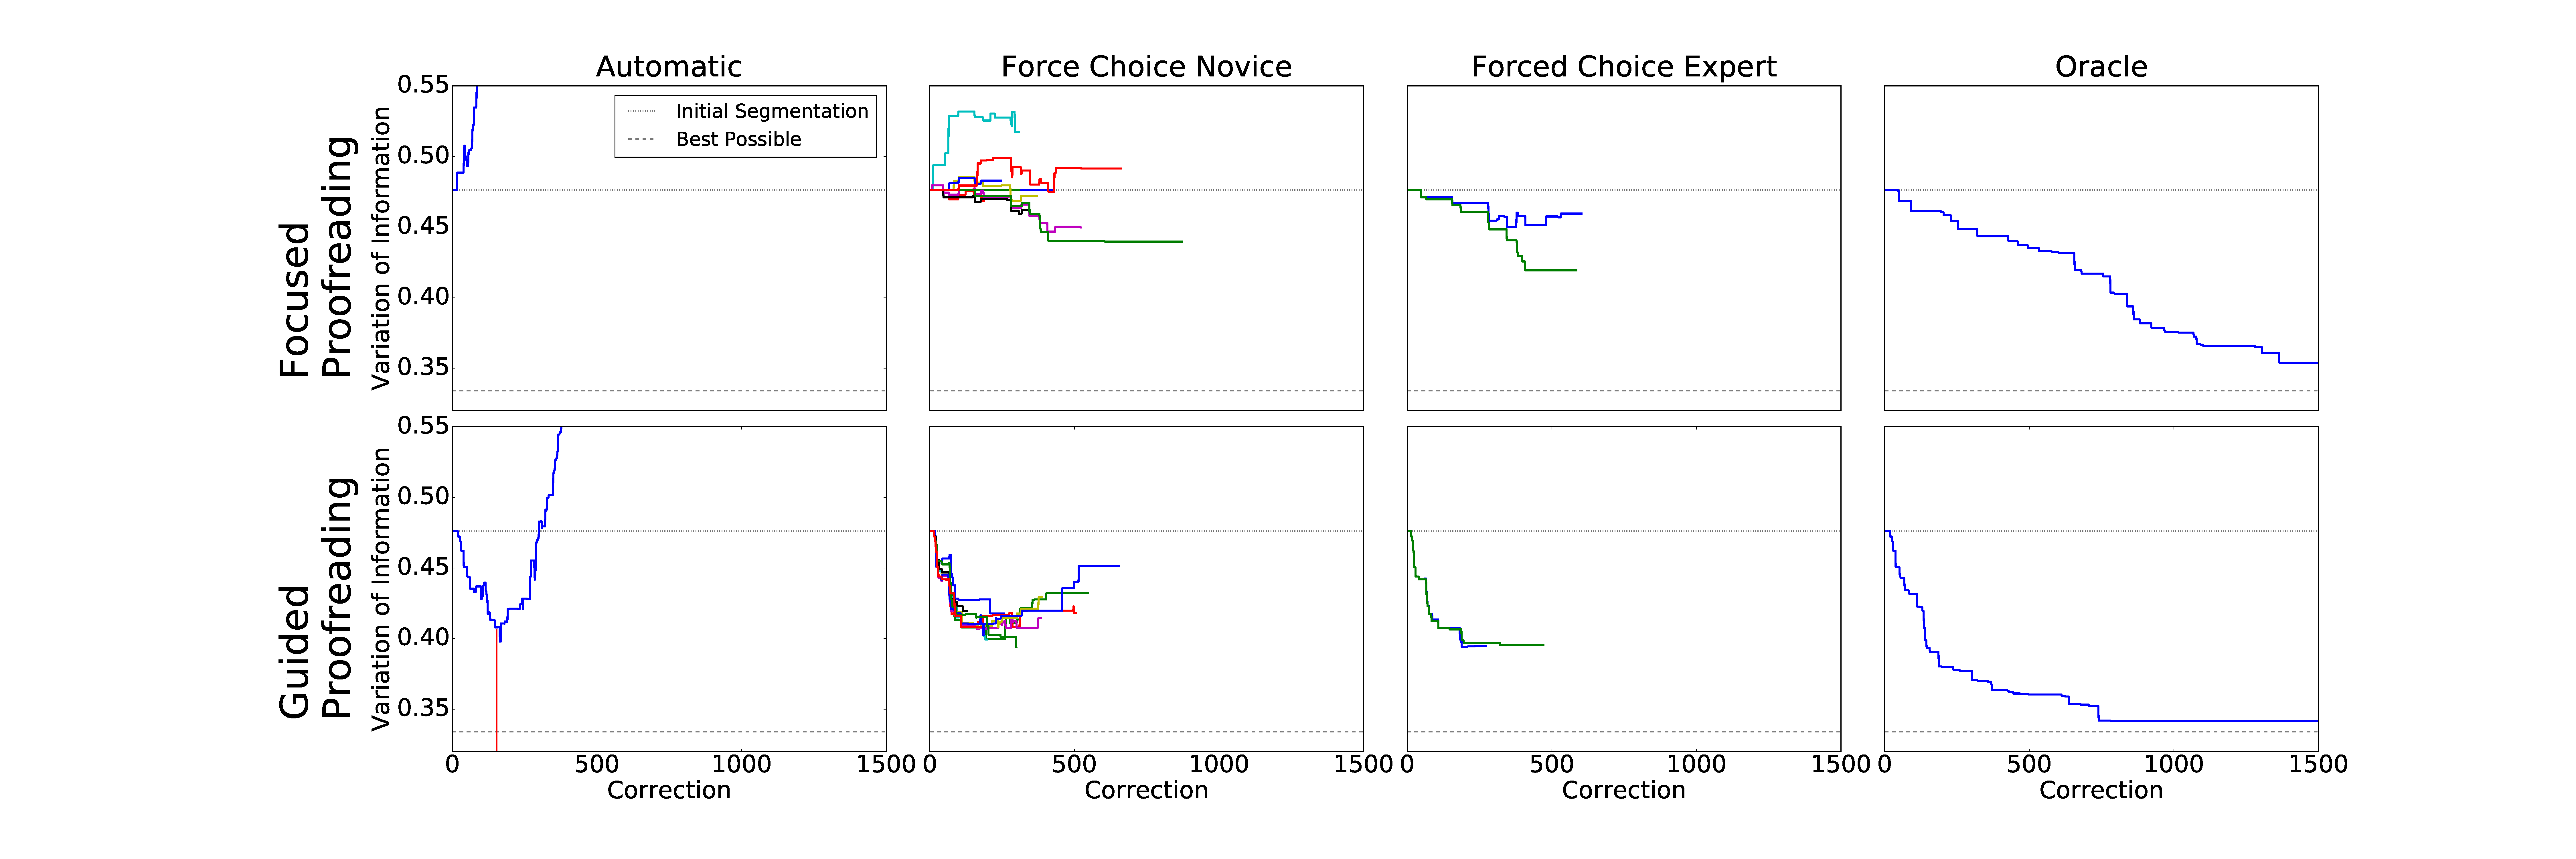
\includegraphics[width=\linewidth]{gfx/ac4trails.pdf}
\end{center}
  \vspace{-4mm}
   \caption{Performance comparison of focused proofreading by Plaza and our guided proofreading methods on the AC4 subvolume. All measurements are reported as median VI, the lower the better. We compare different approaches of accepting or rejecting corrections for each method: automatic selection with threshold (indicated by the red line), forced choice by ten novice users, forced choice by two domain experts, and the selection oracle. In all cases, guided proofreading yields better results with less corrections.}
\label{fig:ac4trails}
\end{figure*}

\begin{figure}[t]
\begin{center}
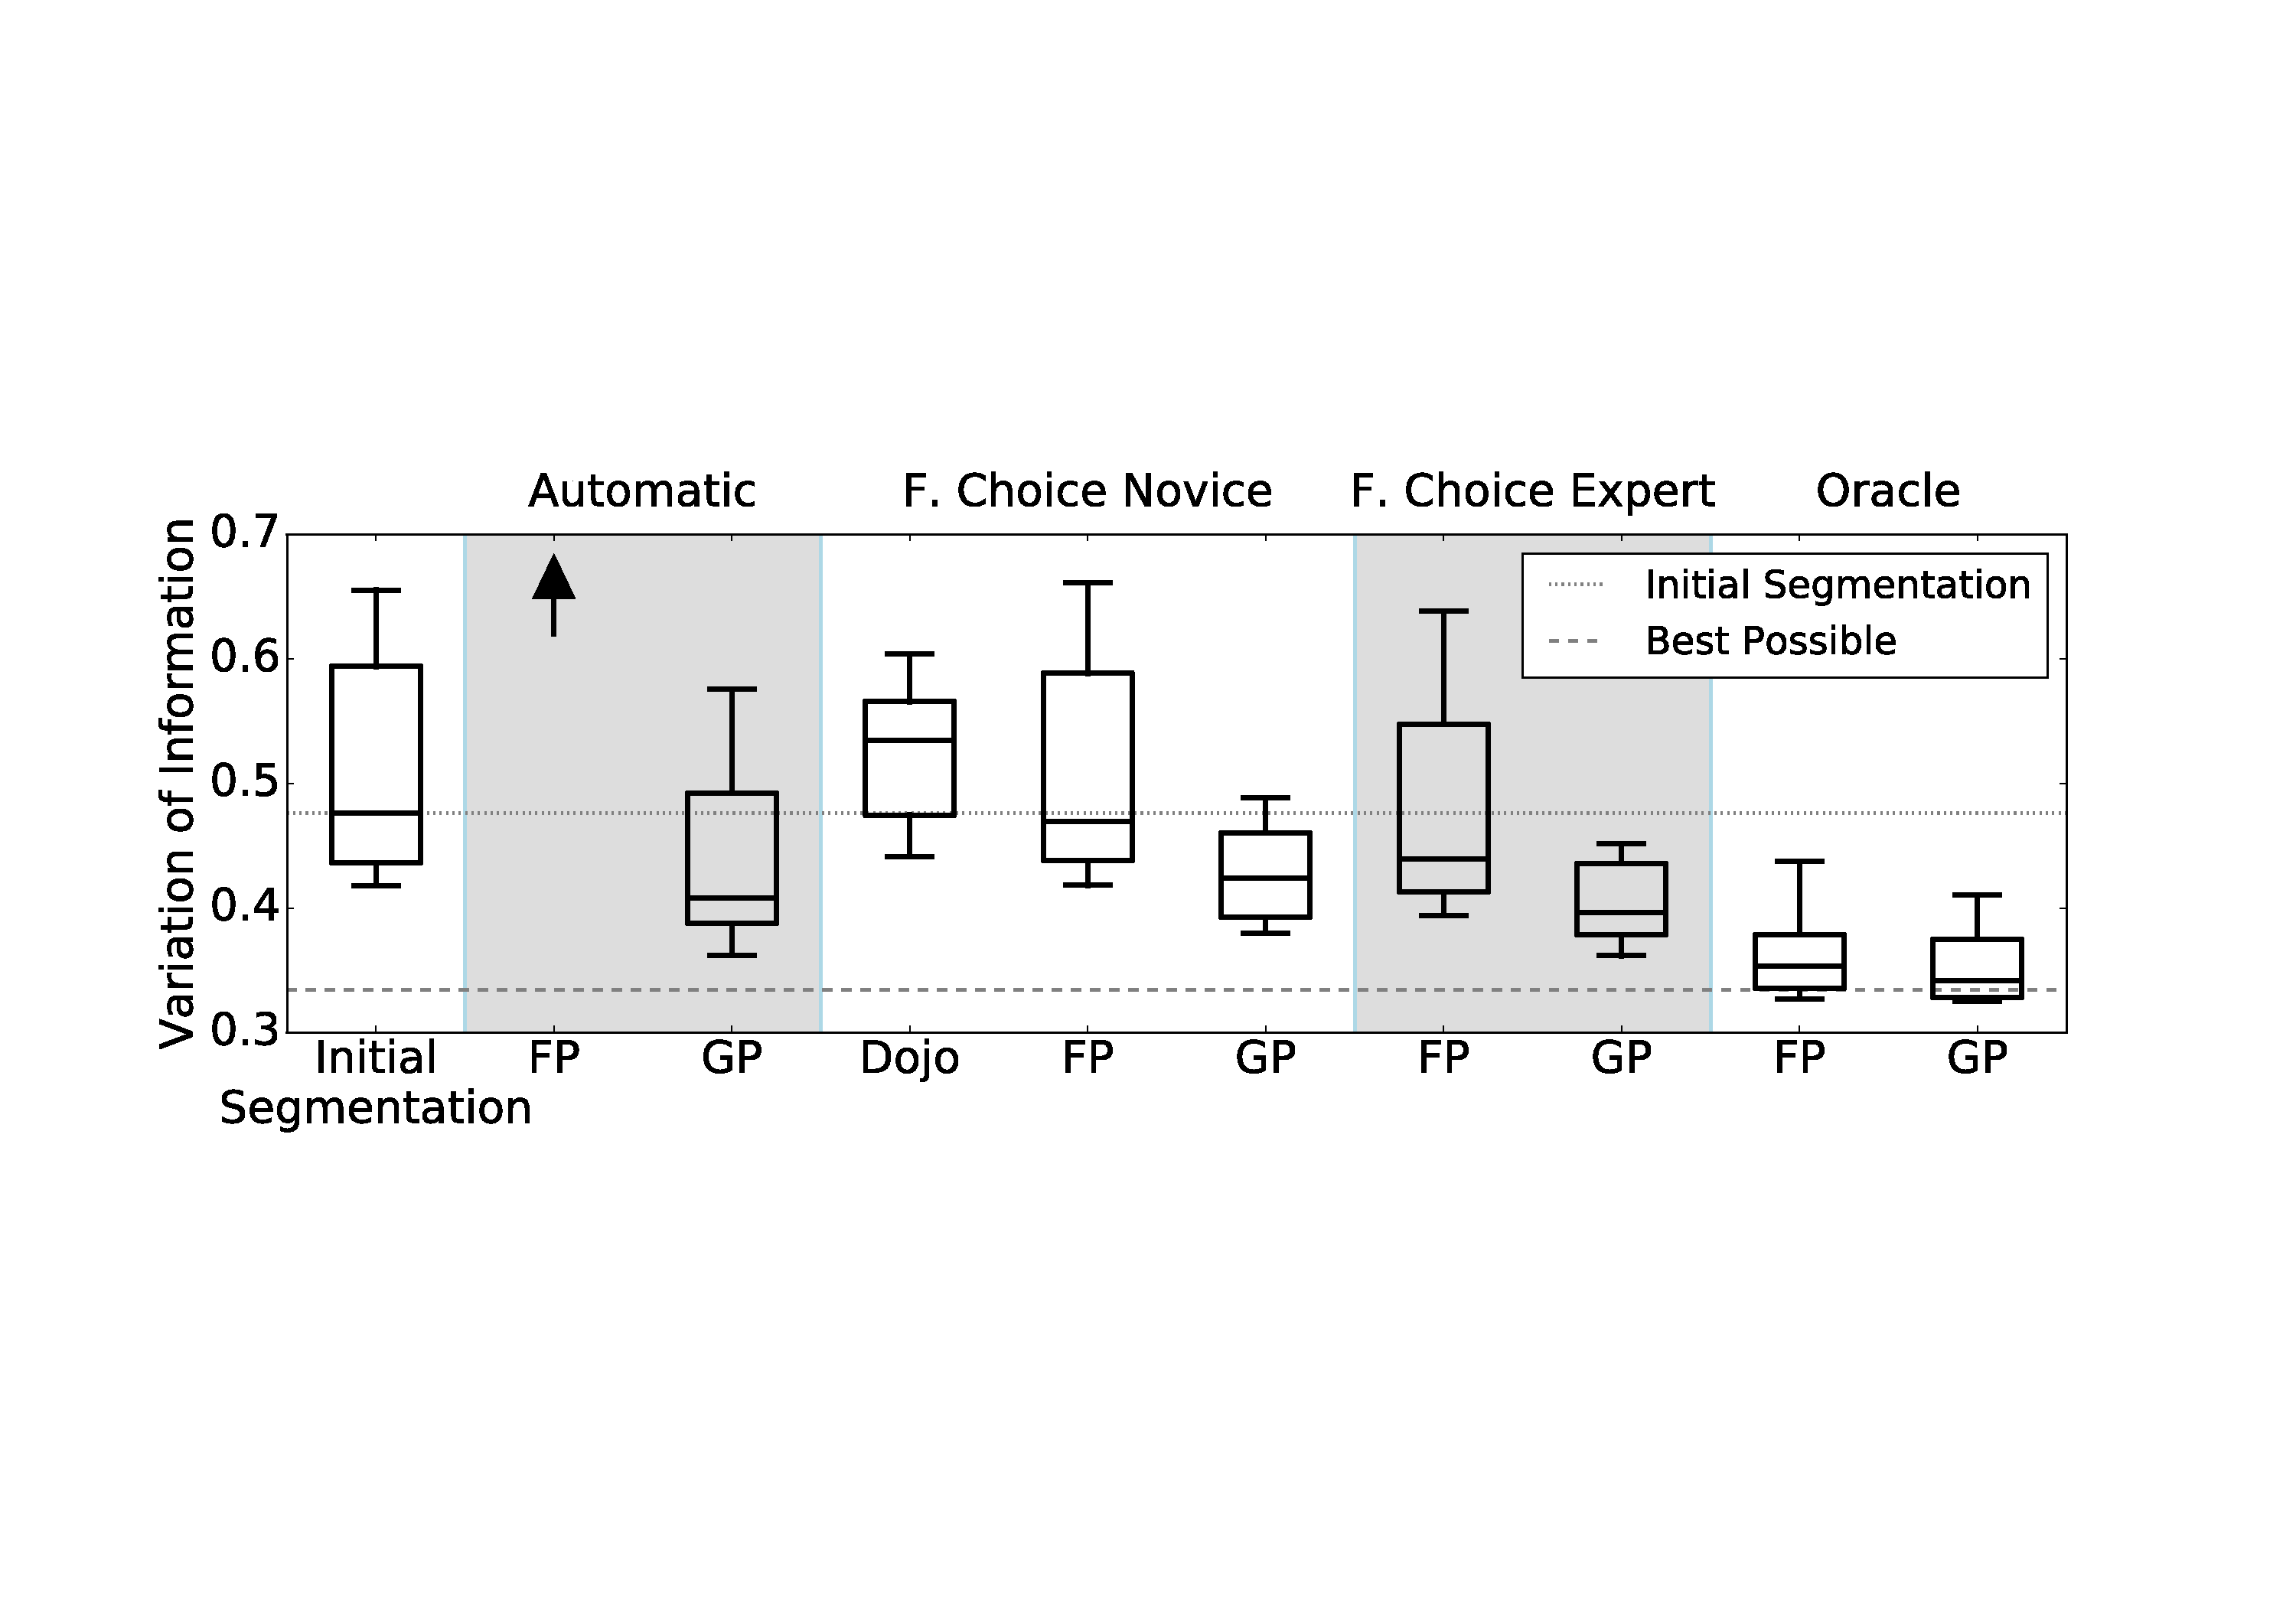
\includegraphics[width=\linewidth]{gfx/ac4boxplot.pdf}
\end{center}
  \vspace{-4mm}
   \caption{VI distributions of proofreading output across ten slices of the AC4 subvolume. The different decision approaches yield different proofreading performances.}
\label{fig:ac4trails}
\end{figure}

\section{Results and Discussion}

%We measure the performance of proofreading quantitatively by comparing VI scores of segmentations against ground truth labelings. Lower VI scores indicate less distance to the ground truth and a better segmentation. For all experiments, we report the VI score of the initial segmentation followed by the VI score of the proofreading output.



\subsection{Selection Oracle}
Accepting and rejecting proofreading corrections with the selection oracle yields the best performance on all datasets. This is not surprising since all detected merge and split are corrected if they are good corrections.


\subsection{Automatic Method}

\subsection{Force Choice User Experiment}

The initial segmentation for AC4 had a VI of XXX. 

\textbf{Novice Performance.} 
\\~\\
\textbf{Expert Performance.}
\\~\\
\textbf{Subjective Responses.} All subjective responses were recorded using the NASA-TLX workload index. The workload index asks study participants to state their mental, physical, temporal demands, as well as rate their performance, effort, and frustration on a scale with 21 graduations. Mental, physical, and temporal demands were reported slightly higher for participants using focused proofreading. However, these differences were not statistically significant. This is not surprising since the user interface was the same for both control groups.
